% ==============================================================
% AERO-GCS FLIGHT ENDURANCE ESTIMATOR — TECHNICAL DOCUMENTATION
% Based on: barebone_template.tex style
% Author: Aadarsh Sinha & Krishnashish Das
% ==============================================================

\documentclass[11pt,a4paper]{article}

% ============================================================
% PACKAGES
% ============================================================
\usepackage[utf8]{inputenc}
\usepackage[T1]{fontenc}
\usepackage{lmodern}
\usepackage[margin=1in]{geometry}
\usepackage{graphicx}
\usepackage{hyperref}
\usepackage{xcolor}
\usepackage{listings}
\usepackage{booktabs}
\usepackage{tabularx}
\usepackage{longtable}
\usepackage{amsmath}
\usepackage{amssymb}
\usepackage{fancyhdr}
\usepackage{titlesec}
\usepackage{enumitem}
\usepackage{tcolorbox}
\usepackage{float}
\usepackage{caption}
\usepackage{subcaption}
\usepackage{multicol}
\usepackage{tikz}
\usetikzlibrary{shapes,arrows,positioning,calc}

% ============================================================
% COLOR DEFINITIONS
% ============================================================
\definecolor{skyblue}{RGB}{0,102,204}
\definecolor{darkblue}{RGB}{0,51,102}
\definecolor{codebg}{RGB}{245,245,245}
\definecolor{codegreen}{RGB}{0,128,0}
\definecolor{codegray}{RGB}{128,128,128}
\definecolor{codepurple}{RGB}{128,0,128}
\definecolor{warnorange}{RGB}{255,140,0}
\definecolor{alertred}{RGB}{204,0,0}
\definecolor{gcscyan}{RGB}{63,214,223}
\definecolor{gcsnavy}{RGB}{10,15,29}
\definecolor{gcsamber}{RGB}{245,166,35}

% ============================================================
% HYPERREF SETUP
% ============================================================
\hypersetup{
    colorlinks=true,
    linkcolor=darkblue,
    urlcolor=skyblue,
    citecolor=darkblue,
    pdftitle={AERO-GCS Flight Endurance Estimator -- Technical Documentation},
    pdfauthor={Aadarsh Sinha and Krishnashish Das},
}

% ============================================================
% CODE LISTING STYLE
% ============================================================
\lstdefinestyle{pythonstyle}{
    backgroundcolor=\color{codebg},
    basicstyle=\ttfamily\footnotesize,
    breaklines=true,
    captionpos=b,
    commentstyle=\color{codegreen},
    keywordstyle=\color{skyblue}\bfseries,
    stringstyle=\color{codepurple},
    numberstyle=\tiny\color{codegray},
    numbers=left,
    numbersep=5pt,
    frame=single,
    rulecolor=\color{codegray},
    language=Python,
    showstringspaces=false,
    tabsize=4,
    morekeywords={async,await,def,class,return,if,else,elif,for,import,from,try,except,finally,raise},
}
\lstset{style=pythonstyle}

% ============================================================
% HEADER / FOOTER
% ============================================================
\setlength{\headheight}{14pt}
\pagestyle{fancy}
\fancyhf{}
\fancyhead[L]{\textcolor{darkblue}{\textbf{AERO-GCS FEE v1.0}}}
\fancyhead[R]{\nouppercase{\leftmark}}
\fancyfoot[L]{\small \copyright\ Wingspann Global}
\fancyfoot[R]{\thepage}
\renewcommand{\headrulewidth}{0.4pt}
\renewcommand{\footrulewidth}{0.4pt}
\renewcommand{\sectionmark}[1]{\markboth{#1}{}}

% ============================================================
% CUSTOM TCOLORBOX ENVIRONMENTS
% ============================================================
\newtcolorbox{notebox}{colback=blue!5!white,colframe=skyblue,title=\textbf{Note},fonttitle=\bfseries}
\newtcolorbox{warnbox}{colback=orange!5!white,colframe=warnorange,title=\textbf{Warning},fonttitle=\bfseries}
\newtcolorbox{alertbox}{colback=red!5!white,colframe=alertred,title=\textbf{Critical},fonttitle=\bfseries}

% ============================================================
% SECTION TITLE FORMATTING
% ============================================================
\titleformat{\section}{\Large\bfseries\color{darkblue}}{\thesection}{1em}{}
\titleformat{\subsection}{\large\bfseries\color{skyblue}}{\thesubsection}{1em}{}
\titleformat{\subsubsection}{\normalsize\bfseries\color{darkblue}}{\thesubsubsection}{1em}{}

% ==============================================================
% DOCUMENT BEGIN
% ==============================================================
\begin{document}

% ============================================================
% TITLE PAGE
% ============================================================
\begin{titlepage}
    \centering
    {
\includegraphics[width=0.5\textwidth]{Icon.png}\par}
    \vspace*{1.5cm}
    {\Huge\bfseries\textcolor{darkblue}{AERO-GCS Flight Endurance Estimator}\par}
    \vspace{0.5cm}
    {\LARGE\textcolor{skyblue}{Version 1.0}\par}
    \vspace{0.3cm}
    {\large\textcolor{codegray}{Technical Documentation \& System Manual}\par}
    \vspace{1.5cm}
    {\large An internal flight-operations tool for estimating drone flight endurance under real-world atmospheric conditions, with telemetry-based model validation and coefficient tuning.\par}
    \vspace{2.5cm}

    {\normalsize
        \textbf{Author:} Aadarsh Sinha \& Krishnashish Das\\
        \textbf{Organization:} Wingspann Global\\[1em]
        \textbf{Document Revision:} 1.0\\
        \vspace{0.8cm}
        \LARGE\textcolor{alertred}{\textbf{Strictly Confidential}}
    }

    \vfill
    {\footnotesize\textcolor{codegray}{This document is a proprietary specification of Wingspann Global. All implementations must conform to the structures described herein. Unauthorized distribution is prohibited.}}
\end{titlepage}

% ============================================================
% DOCUMENT CONTROL
% ============================================================
\newpage
\section*{Document Control}
\addcontentsline{toc}{section}{Document Control}

\begin{table}[H]
    \renewcommand{\arraystretch}{1.5}
    \begin{tabularx}{\textwidth}{@{}lX@{}}
        \toprule
        \textbf{Field} & \textbf{Value} \\
        \midrule
        \textbf{Document Title} & AERO-GCS Flight Endurance Estimator --- Technical Documentation \\
        \textbf{Document ID}    & WG-FEE-DOC-001 \\
        \textbf{Version}        & 1.0 \\
        \textbf{Status}         & Released \\
        \midrule
        \textbf{Author}         & Aadarsh Sinha \& Krishnashish Das \\
        \textbf{Organization}   & Wingspann Global \\
        \midrule
        \textbf{Release Date}   & \today \\
        \textbf{Last Updated}   & \today \\
        \midrule
        \textbf{Distribution}   & Internal Use Only --- Flight Operations Team \\
        \textbf{Classification} & \textcolor{alertred}{\textbf{Strictly Confidential}} \\
        \bottomrule
    \end{tabularx}
\end{table}

\vspace{1cm}

\begin{alertbox}
    \textbf{Document Security Notice:} This document contains proprietary information belonging to Wingspann Global. It is intended exclusively for authorized personnel involved in drone flight operations. Do not copy, distribute, or share this document without explicit written authorization from the engineering team lead.
\end{alertbox}

% ============================================================
% REVISION HISTORY
% ============================================================
\newpage
\section*{Revision History}
\addcontentsline{toc}{section}{Revision History}

\begin{longtable}{@{}p{1.5cm}p{2.5cm}p{3.5cm}p{6cm}@{}}
    \toprule
    \textbf{Version} & \textbf{Date} & \textbf{Author(s)} & \textbf{Changes} \\
    \midrule
    \endfirsthead

    \multicolumn{4}{c}%
    {{\tablename\ \thetable{} -- continued from previous page}} \\
    \toprule
    \textbf{Version} & \textbf{Date} & \textbf{Author(s)} & \textbf{Changes} \\
    \midrule
    \endhead

    \midrule
    \multicolumn{4}{r}{{Continued on next page}} \\
    \endfoot

    \bottomrule
    \endlastfoot

    1.0 & \today & Aadarsh Sinha, Krishnashish Das & Initial document creation. Full system architecture, physics model derivation, UI walkthrough, and deployment guide. \\
    \bottomrule
\end{longtable}

% ============================================================
% TABLE OF CONTENTS
% ============================================================
\newpage
\tableofcontents
\newpage

% ============================================================
% ABSTRACT
% ============================================================
\section*{Abstract}
\markboth{Abstract}{}
\addcontentsline{toc}{section}{Abstract}

The \textbf{AERO-GCS Flight Endurance Estimator} (FEE) is an internal web-based tool developed for the Wingspann Global flight-operations team. It computes the estimated hover endurance and cruise range of multi-rotor UAV platforms under real-world conditions, accounting for battery chemistry, payload mass, ambient temperature, wind loading, and density altitude.

Key features include:
\begin{itemize}[noitemsep]
    \item \textbf{Physics-Based Estimation:} Piecewise LiPo temperature derating, wind-drag current scaling, barometric density-altitude penalties, and momentum-theory payload adjustment.
    \item \textbf{Live Weather Sync:} Integration with the Open-Meteo API (no API key required) for real-time temperature, wind speed, and site elevation, with automatic offline caching.
    \item \textbf{Telemetry Validation:} Flight-log recording against saved aircraft profiles, with predicted-vs-actual scatter regression and tunable model coefficients.
    \item \textbf{GCS-Themed Interface:} Dark navy HUD-style dashboard with JetBrains Mono telemetry readouts, a horizontal derating diagnostics waterfall, and inline safety advisories.
    \item \textbf{Data Export:} Session and flight-log CSV export, plus browser-based PDF report generation.
\end{itemize}

\newpage

% ============================================================
% 1. INTRODUCTION
% ============================================================
\section{Introduction}

\subsection{Problem Statement}
Flight operations teams routinely need to estimate how long a specific drone airframe can remain aloft under a given set of conditions. Off-the-shelf calculators typically apply only a single ``efficiency factor'' and ignore critical environmental variables such as ambient temperature (which affects LiPo internal resistance), wind speed (which increases motor current draw to maintain station), and site altitude (which reduces propeller lift efficiency due to lower air density).

The Flight Endurance Estimator was designed to bridge this gap by providing a multi-variable, physics-grounded model that can be \emph{tuned against real telemetry} rather than trusted blindly.

\subsection{Design Goals}
\begin{enumerate}
    \item \textbf{Accurate, Multi-Variable Physics:} Go beyond simple capacity-over-current calculations by incorporating temperature, wind, altitude, and payload derating curves derived from published LiPo datasheets and aerodynamic theory.
    \item \textbf{Operator-Friendly Interface:} Present results in a GCS-familiar aesthetic (dark background, monospace telemetry fonts, inline advisory banners) so that flight crews can interpret outputs at a glance.
    \item \textbf{Model Calibration:} Allow operators to log actual flight times and adjust model sensitivity coefficients per-aircraft, building confidence in predictions over time.
    \item \textbf{Offline Resilience:} Cache weather readings locally so the tool remains functional in field environments with limited connectivity.
    \item \textbf{Auditability:} Export session data and flight logs as CSV/PDF for inclusion in flight-operations records.
\end{enumerate}

\begin{notebox}
    The estimator is designed as a \textbf{planning aid}, not a safety-of-flight instrument. Operators must always apply their own judgment and adhere to organizational SOPs regarding minimum reserve levels and weather limits.
\end{notebox}

\newpage

% ============================================================
% 2. SYSTEM ARCHITECTURE
% ============================================================
\section{System Architecture}

\subsection{Technology Stack}
The application is built on a two-tier architecture:

\begin{itemize}[noitemsep]
    \item \textbf{Backend:} Python 3.14, FastAPI, SQLAlchemy (ORM), SQLite (persistence), HTTPX (async HTTP client for weather API).
    \item \textbf{Frontend:} Vanilla HTML5, CSS3, and ES6 JavaScript --- no external UI frameworks or charting libraries. Custom SVG rendering for all charts.
    \item \textbf{Deployment:} Uvicorn ASGI server, single \texttt{run.bat} bootstrap launcher.
\end{itemize}

\subsection{System Architecture Diagram}

\begin{figure}[H]
    \centering
    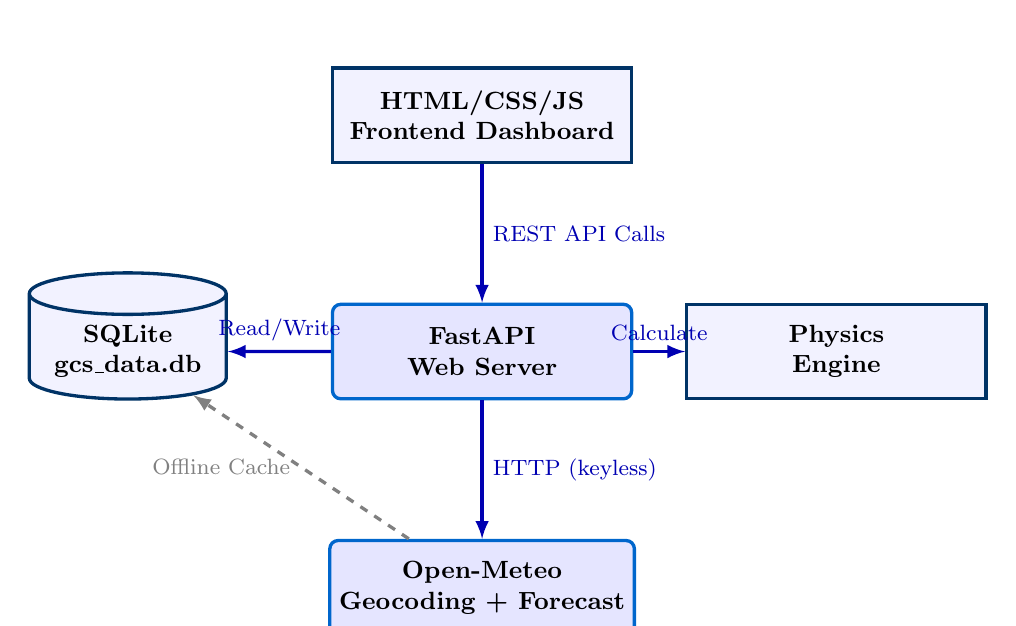
\begin{tikzpicture}[
        box/.style={rectangle, draw=darkblue, very thick, minimum width=3.8cm, minimum height=1.2cm, align=center, fill=blue!5!white, font=\small\bfseries},
        db/.style={cylinder, draw=darkblue, very thick, minimum width=2.5cm, minimum height=1.5cm, shape border rotate=90, aspect=0.25, fill=blue!5!white, font=\small\bfseries, align=center},
        api/.style={rectangle, draw=skyblue, very thick, minimum width=3.8cm, minimum height=1.2cm, align=center, fill=blue!10!white, font=\small\bfseries, rounded corners=3pt},
        arrow/.style={->, very thick, >=latex, line width=1.2pt}]

        \node[box] (ui) at (0,0) {HTML/CSS/JS\\Frontend Dashboard};
        \node[api] (fastapi) at (0,-3) {FastAPI\\Web Server};
        \node[db] (sqlite) at (-4.5,-3) {SQLite\\gcs\_data.db};
        \node[box] (physics) at (4.5,-3) {Physics\\Engine};
        \node[api] (weather) at (0,-6) {Open-Meteo\\Geocoding + Forecast};

        \draw[arrow, blue!70!black] (ui) -- node[right, font=\footnotesize]{REST API Calls} (fastapi);
        \draw[arrow, blue!70!black] (fastapi) -- node[above, font=\footnotesize]{Read/Write} (sqlite);
        \draw[arrow, blue!70!black] (fastapi) -- node[above, font=\footnotesize]{Calculate} (physics);
        \draw[arrow, blue!70!black] (fastapi) -- node[right, font=\footnotesize]{HTTP (keyless)} (weather);
        \draw[arrow, codegray, dashed] (weather) -- node[left, font=\footnotesize]{Offline Cache} (sqlite);

    \end{tikzpicture}
    \caption{AERO-GCS Flight Endurance Estimator --- System Architecture}
\end{figure}

\subsection{Directory Structure}

\begin{table}[H]
    \centering
    \begin{tabularx}{\textwidth}{@{}lX@{}}
        \toprule
        \textbf{Path} & \textbf{Description} \\
        \midrule
        \texttt{backend/main.py} & FastAPI application entry point. Defines all REST API endpoints, CORS middleware, and mounts static frontend files. \\
        \texttt{backend/database.py} & SQLAlchemy engine, session factory, and SQLite foreign-key enforcement. \\
        \texttt{backend/models.py} & ORM models: \texttt{Aircraft}, \texttt{FlightLog}, \texttt{WeatherCache}. \\
        \texttt{backend/schemas.py} & Pydantic request/response validation schemas. \\
        \texttt{backend/physics.py} & Core derating calculations (temperature, wind, altitude, payload). \\
        \texttt{backend/weather.py} & Open-Meteo API integration with geocoding and offline caching. \\
        \texttt{backend/test\_physics.py} & Automated unit tests for all physics calculations. \\
        \texttt{backend/test\_api.py} & Automated API integration tests. \\
        \midrule
        \texttt{frontend/index.html} & Single-page application structure. \\
        \texttt{frontend/css/style.css} & AERO-GCS dark navy theme, responsive layout, print stylesheet. \\
        \texttt{frontend/js/api.js} & REST client wrapper (fetch-based). \\
        \texttt{frontend/js/app.js} & UI state management, form handlers, real-time calculation mirror. \\
        \texttt{frontend/js/charts.js} & Custom SVG waterfall and scatter-plot renderers. \\
        \midrule
        \texttt{run.bat} & Windows bootstrap launcher (activates venv, starts Uvicorn on port 7006). \\
        \texttt{gcs\_data.db} & SQLite database file (auto-created on first run). \\
        \bottomrule
    \end{tabularx}
    \caption{Project File Structure}
\end{table}

\newpage

% ============================================================
% 3. DATABASE SCHEMA
% ============================================================
\section{Database Schema}

The application uses SQLite via SQLAlchemy. Three tables persist all operational data.

\subsection{Aircraft Table}
Stores saved drone configuration profiles. Each profile includes physical specifications, battery parameters, and per-aircraft tuning coefficients.

\begin{table}[H]
    \centering
    \renewcommand{\arraystretch}{1.3}
    \begin{tabularx}{\textwidth}{@{}llX@{}}
        \toprule
        \textbf{Column} & \textbf{Type} & \textbf{Description} \\
        \midrule
        \texttt{id} & INTEGER PK & Auto-incrementing identifier \\
        \texttt{name} & TEXT UNIQUE & Human-readable aircraft identifier \\
        \texttt{empty\_weight} & REAL & Airframe weight without payload (kg) \\
        \texttt{motors} & INTEGER & Number of motors \\
        \texttt{hover\_current} & REAL & Measured hover current per motor at empty weight (A) \\
        \texttt{prop\_size} & TEXT & Propeller dimensions (e.g., ``15x5.2'') \\
        \texttt{battery\_capacity} & INTEGER & Battery capacity (mAh) \\
        \texttt{battery\_cells} & INTEGER & Cell count (S) \\
        \texttt{battery\_reserve} & REAL & Land-with reserve percentage \\
        \texttt{battery\_efficiency} & REAL & Discharge efficiency percentage \\
        \texttt{cruise\_speed} & REAL & Optional cruise speed (km/h) \\
        \texttt{temp\_coeff} & REAL & Temperature sensitivity coefficient (default 1.0) \\
        \texttt{wind\_coeff} & REAL & Wind sensitivity coefficient (default 1.0) \\
        \texttt{alt\_coeff} & REAL & Altitude sensitivity coefficient (default 1.0) \\
        \texttt{created\_at} & DATETIME & Profile creation timestamp \\
        \bottomrule
    \end{tabularx}
    \caption{Aircraft Profile Table Schema}
\end{table}

\subsection{FlightLog Table}
Records of actual flights with measured conditions and duration, linked to an aircraft profile via foreign key.

\subsection{WeatherCache Table}
Stores the last-fetched weather reading per location (keyed by place name or coordinate pair). Used for offline fallback when the Open-Meteo API is unreachable.

\newpage

% ============================================================
% 4. PHYSICS MODEL
% ============================================================
\section{Physics Model --- Flight Endurance Calculation}

The estimator applies a cascading series of derating factors to the theoretical nameplate hover time. Each stage is displayed in the UI as a step in the ``derating waterfall'' diagnostics panel.

\subsection{Stage 1: Payload Current Scaling}
Using momentum theory, hover current scales non-linearly with total weight:

\begin{equation}
    I_{\text{hover}} = I_{\text{hover, empty}} \times \left(\frac{W_{\text{empty}} + W_{\text{payload}}}{W_{\text{empty}}}\right)^{1.3}
\end{equation}

The exponent of 1.3 is derived from the relationship between thrust, power, and rotor disc loading in momentum theory. If no payload is specified, the scale factor defaults to 1.0.

\subsection{Stage 2: Nameplate Hover Time}
The theoretical maximum hover time at the loaded current draw:

\begin{equation}
    t_{\text{nameplate}} = \frac{C_{\text{mAh}} / 1000}{N_{\text{motors}} \times I_{\text{hover}}} \times 60 \quad \text{[minutes]}
\end{equation}

\subsection{Stage 3: Usable Capacity Limit}
Accounting for the land-with reserve and discharge efficiency losses:

\begin{equation}
    t_{\text{usable}} = t_{\text{nameplate}} \times \left(1 - \frac{R_{\text{reserve}}}{100}\right) \times \frac{\eta_{\text{efficiency}}}{100}
\end{equation}

\subsection{Stage 4: LiPo Temperature Derating}
A piecewise function models the capacity reduction due to battery temperature:

\begin{equation}
    d_{\text{temp}}(T) =
    \begin{cases}
        0.50 & T \leq -20^{\circ}\text{C} \\
        0.50 + 0.50 \times \dfrac{T + 20}{40} & -20^{\circ}\text{C} < T < 20^{\circ}\text{C} \\
        1.00 & 20^{\circ}\text{C} \leq T \leq 35^{\circ}\text{C} \\
        1.00 - 0.15 \times \dfrac{T - 35}{20} & 35^{\circ}\text{C} < T \leq 55^{\circ}\text{C} \\
        0.85 & T > 55^{\circ}\text{C}
    \end{cases}
\end{equation}

Applied with the tunable sensitivity coefficient $C_{\text{temp}}$:
\begin{equation}
    d_{\text{temp, adj}} = 1.0 - (1.0 - d_{\text{temp}}) \times C_{\text{temp}}
\end{equation}
\begin{equation}
    t_{\text{temp}} = t_{\text{usable}} \times d_{\text{temp, adj}}
\end{equation}

\begin{warnbox}
    At temperatures below $0^{\circ}$C, LiPo cells suffer significant internal resistance increases and voltage sag. The estimator will surface an inline advisory recommending battery pre-heating before takeoff.
\end{warnbox}

\subsection{Stage 5: Wind Current Penalty}
Motor current draw increases to maintain station in wind. The penalty is modeled as a piecewise linear function:

\begin{equation}
    p_{\text{wind}}(W) =
    \begin{cases}
        1.00 & W \leq 10 \text{ km/h} \\
        1.00 + 0.65 \times \dfrac{W - 10}{40} & 10 < W \leq 50 \text{ km/h} \\
        1.65 & W > 50 \text{ km/h}
    \end{cases}
\end{equation}

Applied with tuning coefficient:
\begin{equation}
    p_{\text{wind, adj}} = 1.0 + (p_{\text{wind}} - 1.0) \times C_{\text{wind}}
\end{equation}
\begin{equation}
    t_{\text{wind}} = t_{\text{temp}} \,/\, p_{\text{wind, adj}}
\end{equation}

\subsection{Stage 6: Density Altitude Penalty}
At higher altitudes, air density decreases, requiring higher motor RPM (and thus more current) to produce the same thrust:

\begin{equation}
    \rho_{\text{ratio}} = \exp\left(-\frac{\text{altitude}}{8500}\right)
\end{equation}
\begin{equation}
    p_{\text{alt}} = \frac{1}{\sqrt{\rho_{\text{ratio}}}} = \exp\left(\frac{\text{altitude}}{17000}\right)
\end{equation}
\begin{equation}
    t_{\text{final}} = t_{\text{wind}} \,/\, p_{\text{alt, adj}}
\end{equation}

\subsection{Range Estimation}
If a cruise speed $v_{\text{cruise}}$ is provided:
\begin{equation}
    R_{\text{range}} = \frac{t_{\text{final}}}{60} \times v_{\text{cruise}} \quad \text{[km]}
\end{equation}

\subsection{Safety Advisories}
The system surfaces non-blocking inline advisories (not modal dialogs) when:
\begin{itemize}[noitemsep]
    \item Wind speed exceeds 25 km/h (\textcolor{gcsamber}{warning}) or 40 km/h (\textcolor{alertred}{critical})
    \item Temperature is below $0^{\circ}$C or above $45^{\circ}$C (\textcolor{gcsamber}{warning})
    \item Site altitude exceeds 3000 m (\textcolor{gcsamber}{warning})
    \item Estimated flight time is under 3 minutes (\textcolor{alertred}{critical})
\end{itemize}

\newpage

% ============================================================
% 5. WEATHER INTEGRATION
% ============================================================
\section{Weather Integration}

\subsection{Open-Meteo API}
The system uses the \href{https://open-meteo.com/}{Open-Meteo} forecast and geocoding APIs, which require no API key. This eliminates credential management overhead for field deployments.

\begin{description}[style=nextline]
    \item[\textbf{Geocoding API}] Resolves place names (e.g., ``San Francisco, CA'') to latitude/longitude coordinates. Returns the official place name, administrative region, and elevation.
    \item[\textbf{Forecast API}] Returns current conditions for given coordinates: \texttt{temperature\_2m}, \texttt{wind\_speed\_10m}, \texttt{relative\_humidity\_2m}, and site \texttt{elevation}.
\end{description}

\subsection{Offline Caching Strategy}
Every successful weather fetch is persisted to the \texttt{WeatherCache} table under three keys:
\begin{enumerate}[noitemsep]
    \item \texttt{last\_fetched} --- always overwritten with the most recent query.
    \item \texttt{coord:\{lat\},\{lon\}} --- keyed by rounded coordinates for coordinate-based lookups.
    \item \texttt{name:\{query\}} --- keyed by the search term for name-based lookups.
\end{enumerate}

If the API is unreachable, the system attempts cache recovery in order: specific coordinate/name cache first, then the global \texttt{last\_fetched} entry. If no cache exists, a clear error message instructs the operator to enter conditions manually.

\newpage

% ============================================================
% 6. USER INTERFACE
% ============================================================
\section{User Interface}

The frontend follows the AERO-GCS ground control station visual language: dark navy backgrounds, cyan accent colors, JetBrains Mono for telemetry data, Inter for labels, and an industrial, panel-based layout.

\subsection{Dashboard Overview}

\begin{figure}[H]
    \centering
    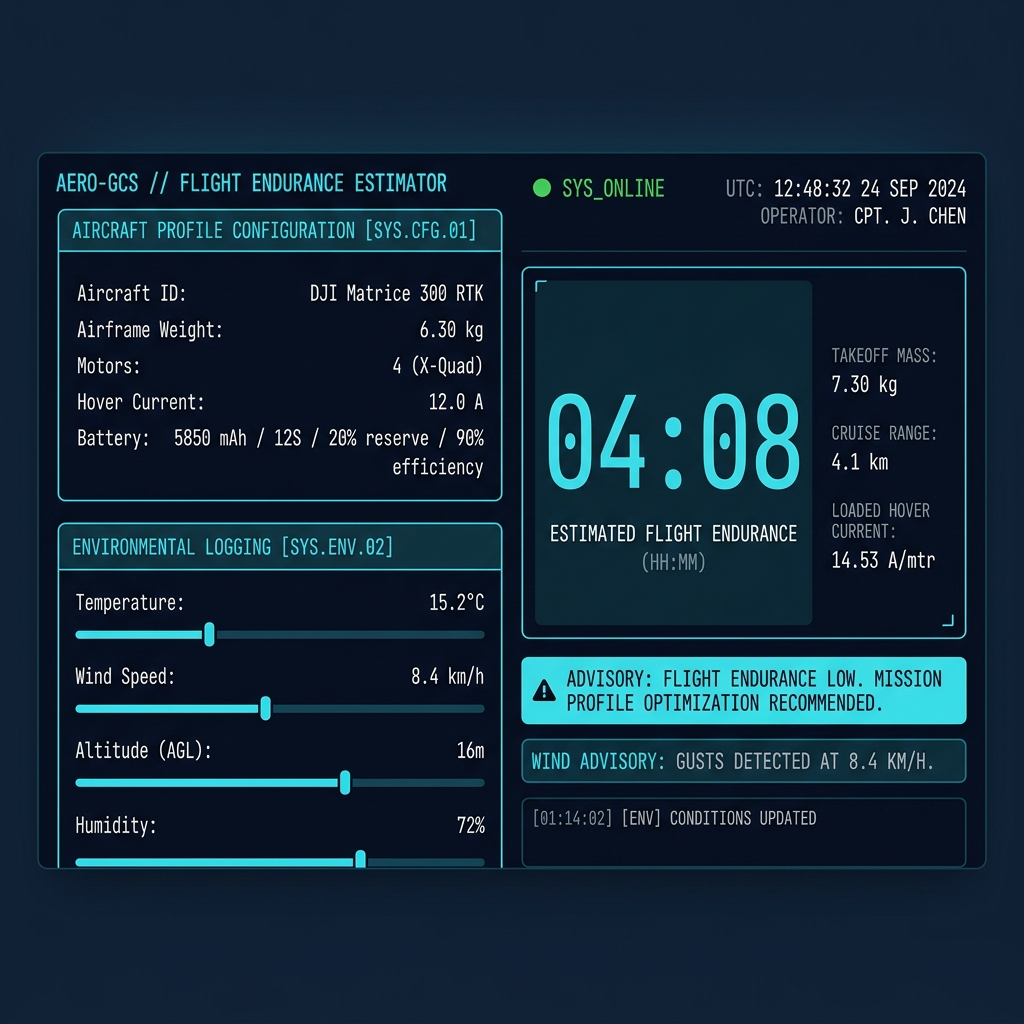
\includegraphics[width=\textwidth]{screenshot_dashboard.png}
    \caption{AERO-GCS Flight Endurance Estimator --- Main Dashboard View. The left column contains the aircraft profile configuration and environmental controls. The right column displays the HUD timer, advisories, waterfall diagnostics, and model tuning panels.}
\end{figure}

\subsection{HUD Flight Timer}
The primary output is a large, monospace digital readout displaying the estimated flight endurance in \texttt{MM:SS} format. This readout updates in real-time as sliders and inputs are adjusted. Secondary telemetry values (takeoff mass, cruise range, loaded hover current) are displayed alongside.

\subsection{Derating Waterfall Diagnostics}

\begin{figure}[H]
    \centering
    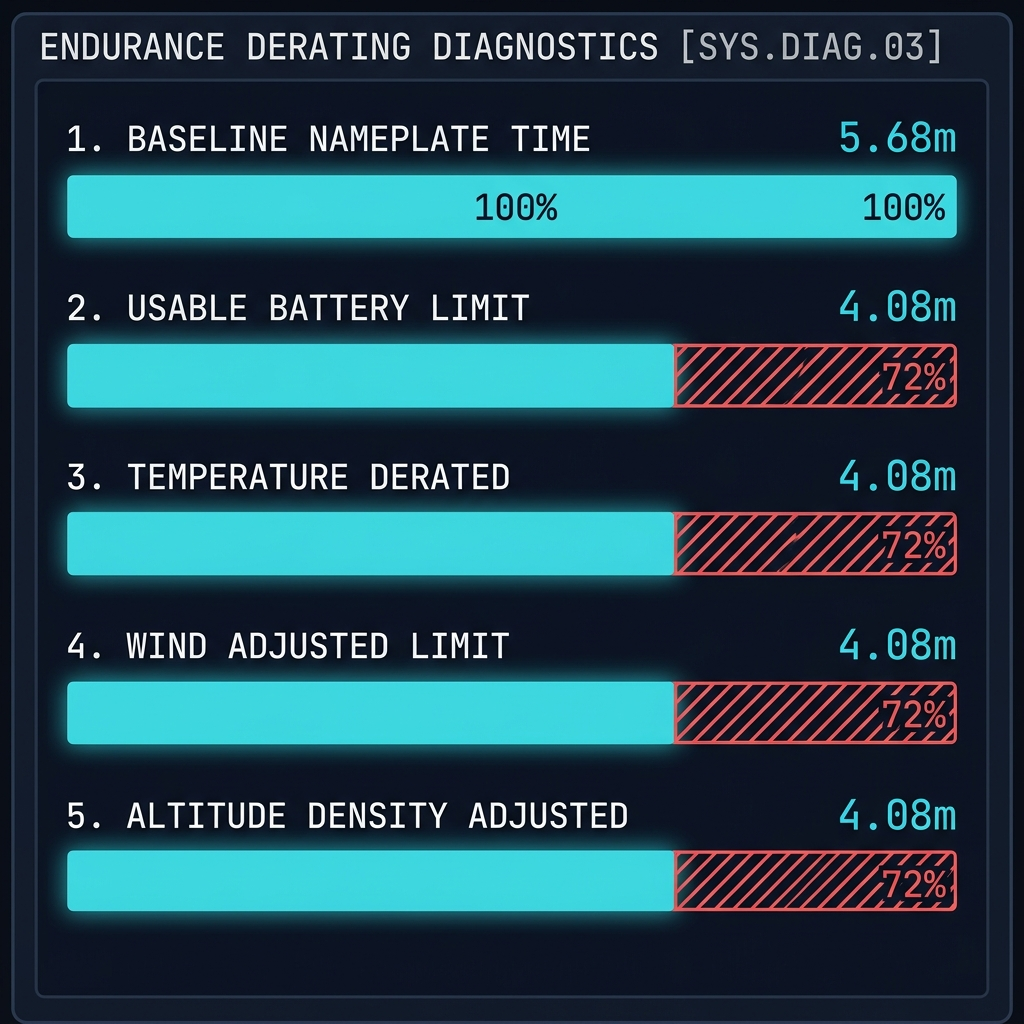
\includegraphics[width=\textwidth]{screenshot_waterfall.png}
    \caption{Endurance Derating Diagnostics --- Horizontal step-bar waterfall showing progressive capacity reduction through each derating stage. Cyan bars represent remaining capacity; hatched sections indicate losses.}
\end{figure}

The waterfall reads like a GCS diagnostics panel rather than a generic chart. Each row shows:
\begin{itemize}[noitemsep]
    \item The stage label (e.g., ``2. USABLE BATTERY LIMIT'')
    \item The resulting flight time and percentage of nameplate remaining
    \item A horizontal bar proportional to the nameplate time, with the loss portion rendered as a hatched overlay
\end{itemize}

\subsection{Model Tuning \& Coefficient Regression}

\begin{figure}[H]
    \centering
    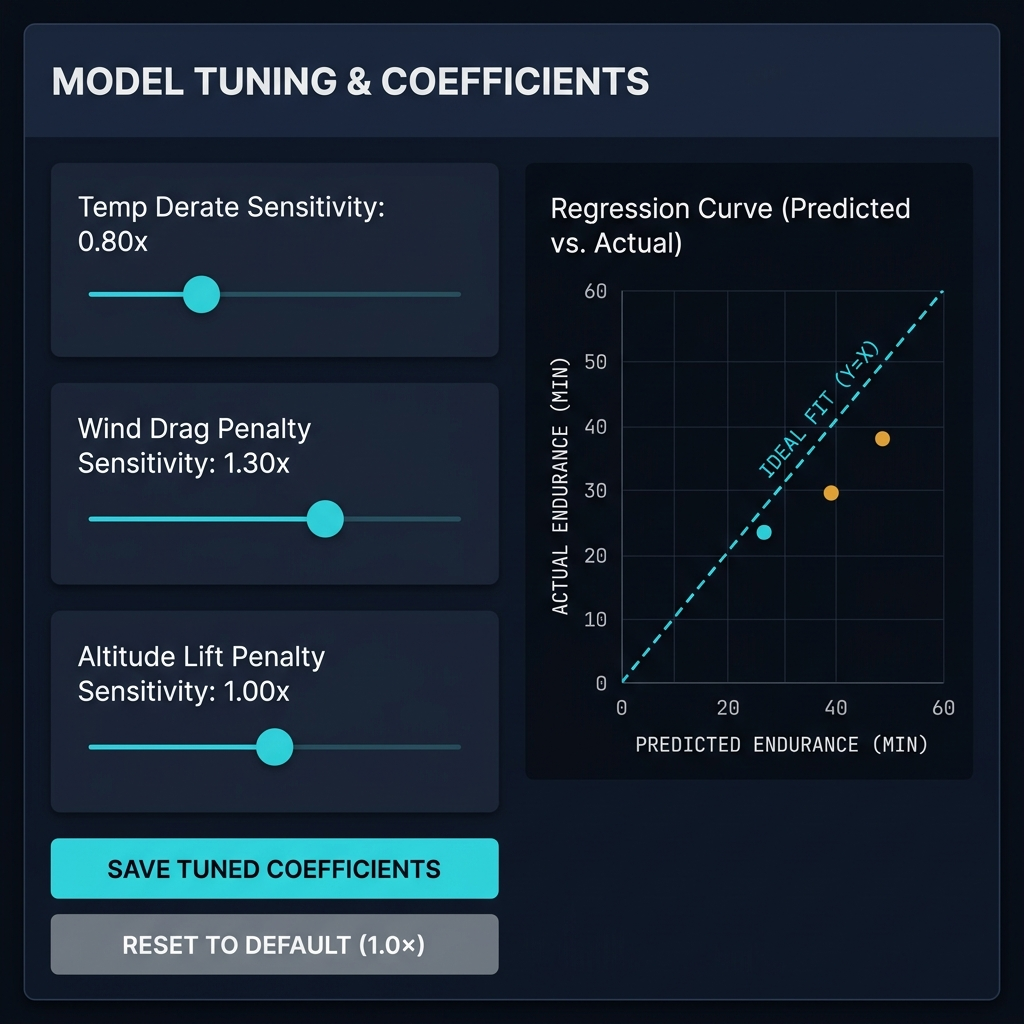
\includegraphics[width=\textwidth]{screenshot_tuning.png}
    \caption{Model Tuning Panel --- Sensitivity coefficient sliders (left) and predicted-vs-actual scatter regression plot (right). Dots are color-coded by prediction accuracy: cyan ($<$15\% error), amber (15--30\%), red ($>$30\%).}
\end{figure}

The tuning panel allows operators to adjust three coefficients per aircraft:
\begin{itemize}[noitemsep]
    \item \textbf{Temperature Derate Sensitivity} ($C_{\text{temp}}$): Amplifies or reduces the LiPo temperature penalty.
    \item \textbf{Wind Drag Penalty Sensitivity} ($C_{\text{wind}}$): Amplifies or reduces the wind current scaling.
    \item \textbf{Altitude Lift Penalty Sensitivity} ($C_{\text{alt}}$): Amplifies or reduces the density altitude effect.
\end{itemize}

As sliders are dragged, the scatter plot updates at 60~fps using a client-side JavaScript mirror of the backend physics calculations. This allows operators to visually align prediction dots with the ideal $y = x$ regression line before saving coefficients to the aircraft profile.

\subsection{Flight Logs \& Validation Table}
The ``Flight Op Logs \& Validation'' tab provides:
\begin{itemize}[noitemsep]
    \item A log submission form that auto-captures current environmental slider values as flight conditions.
    \item A scrollable table showing all logged flights with columns: Date, Payload, Environment (T/W/A), Actual time, Predicted time, and prediction error percentage.
    \item CSV export of the full log history for a selected aircraft.
\end{itemize}

\newpage

% ============================================================
% 7. API REFERENCE
% ============================================================
\section{API Reference}

All endpoints are served by FastAPI on \texttt{http://localhost:7006}. Interactive Swagger documentation is available at \texttt{/docs}.

\begin{table}[H]
    \centering
    \renewcommand{\arraystretch}{1.4}
    \begin{tabularx}{\textwidth}{@{}llX@{}}
        \toprule
        \textbf{Method} & \textbf{Endpoint} & \textbf{Description} \\
        \midrule
        POST & \texttt{/api/aircraft} & Create a new aircraft profile. \\
        GET & \texttt{/api/aircraft} & List all saved aircraft profiles. \\
        GET & \texttt{/api/aircraft/\{id\}} & Retrieve a specific aircraft profile. \\
        PUT & \texttt{/api/aircraft/\{id\}} & Update aircraft specifications. \\
        PUT & \texttt{/api/aircraft/\{id\}/coefficients} & Update tuning coefficients only. \\
        DELETE & \texttt{/api/aircraft/\{id\}} & Delete profile and all linked logs. \\
        \midrule
        POST & \texttt{/api/flight-logs} & Record a new flight log entry. \\
        GET & \texttt{/api/flight-logs/\{aircraft\_id\}} & List logs for a specific aircraft. \\
        DELETE & \texttt{/api/flight-logs/\{log\_id\}} & Delete a flight log entry. \\
        \midrule
        GET & \texttt{/api/weather?q=\{name\}} & Fetch weather by place name. \\
        GET & \texttt{/api/weather?lat=\{lat\}\&lon=\{lon\}} & Fetch weather by coordinates. \\
        \midrule
        POST & \texttt{/api/estimate} & Run endurance calculation. \\
        GET & \texttt{/api/export/csv?aircraft\_id=\{id\}} & Export flight logs as CSV. \\
        GET & \texttt{/api/export/session-csv?\ldots} & Export session inputs + result as CSV. \\
        \bottomrule
    \end{tabularx}
    \caption{REST API Endpoint Summary}
\end{table}

\newpage

% ============================================================
% 8. TESTING & VALIDATION
% ============================================================
\section{Testing \& Validation}

\subsection{Unit Tests --- Physics Engine}
The file \texttt{backend/test\_physics.py} contains automated assertions for all piecewise curves:

\begin{lstlisting}[caption={Physics test execution output}]
==================================================
 RUNNING FLIGHT ENDURANCE ESTIMATOR PHYSICS TESTS
==================================================
Testing LiPo Temperature Derating Curve...
[PASS] LiPo Temperature curves verified.
Testing Wind Drag Penalty Curve...
[PASS] Wind Drag penalties verified.
Testing Density Altitude Penalty Curve...
[PASS] Density Altitude scaling verified.
Testing Full Estimation Model Calculations...
[PASS] Full estimation model math verified.
Testing Tuning Coefficient Effects...
[PASS] Sensitivity coefficient overrides verified.
==================================================
           ALL TESTS COMPLETED SUCCESS
==================================================
\end{lstlisting}

\subsection{Integration Tests --- API Endpoints}
The file \texttt{backend/test\_api.py} performs end-to-end validation:

\begin{lstlisting}[caption={API integration test execution output}]
==================================================
 RUNNING INTEGRATION TESTS FOR API ON PORT 7006
==================================================
[INFO] Creating aircraft profile...
[PASS] Profile saved successfully with ID: 2
[INFO] Querying /api/estimate endpoint...
[INFO] API Estimation Results:
  - Final Estimated Time: 4.08 mins
  - Loaded Hover Current: 14.53 A/motor
  - Cruise Range: 4.08 km
  - Number of Advisories: 0
[INFO] Cleaning up test profile...
==================================================
    SUCCESS: API INTEGRATION TESTS PASSED!
==================================================
\end{lstlisting}

\newpage

% ============================================================
% 9. DEPLOYMENT
% ============================================================
\section{Deployment \& Usage}

\subsection{Prerequisites}
\begin{itemize}[noitemsep]
    \item Python 3.10 or later
    \item Internet connection for initial dependency installation and weather sync (optional after first use)
\end{itemize}

\subsection{Installation}
\begin{enumerate}
    \item Clone or copy the project directory to the target machine.
    \item Open a terminal in the project root and run:
\begin{lstlisting}[language=bash, caption={Virtual environment setup}]
python -m venv .venv
.venv\Scripts\pip install -r backend\requirements.txt
\end{lstlisting}
\end{enumerate}

\subsection{Running the Application}
Double-click \texttt{run.bat} or execute it from a terminal. The console will display:

\begin{lstlisting}[language=bash, caption={Application startup output}]
==================================================
  AERO-GCS FLIGHT ENDURANCE ESTIMATOR BOOTSTRAP
  Developed by Aadarsh Sinha & Krishnashish Das
==================================================

[INFO] Starting FastAPI App server...
[INFO] Service will be available at http://localhost:7006/
\end{lstlisting}

The browser will automatically open to \texttt{http://localhost:7006/}.

\subsection{Typical Workflow}
\begin{enumerate}
    \item \textbf{Create/Select Aircraft:} Enter airframe specs and save, or select a previously saved profile from the dropdown.
    \item \textbf{Set Environment:} Use the weather sync to pull live conditions, or manually adjust the temperature, wind, altitude, and humidity sliders.
    \item \textbf{Read Results:} The HUD timer, waterfall, and advisories update in real-time.
    \item \textbf{Log Flights:} After a real flight, record the actual duration in the Flight Logs tab. The system auto-captures the current environmental slider values.
    \item \textbf{Tune Model:} Switch to the Model Tuning tab and adjust coefficients until predicted times align with logged actuals on the scatter plot. Save coefficients to the profile.
    \item \textbf{Export:} Download session CSV or print a PDF report for flight-ops records.
\end{enumerate}

\newpage

% ============================================================
% 10. SECURITY CONSIDERATIONS
% ============================================================
\section{Security Considerations}

\begin{alertbox}
    The AERO-GCS Flight Endurance Estimator is designed for internal use on trusted networks. It does not implement authentication or authorization.
\end{alertbox}

\subsection{Operational Constraints}
\begin{itemize}[noitemsep]
    \item \textbf{Network Binding:} The server binds to \texttt{127.0.0.1} by default, restricting access to the local machine only.
    \item \textbf{No External Data Ingestion:} The only outbound connections are to Open-Meteo (a public, keyless API). No user data is transmitted externally.
    \item \textbf{SQLite File Security:} The \texttt{gcs\_data.db} file contains aircraft configurations and flight logs. Protect it according to your organization's data classification policy.
    \item \textbf{Input Validation:} All API inputs are validated by Pydantic schemas with strict range constraints (e.g., temperature $-50^{\circ}$C to $70^{\circ}$C, wind 0--150 km/h).
\end{itemize}

\newpage

% ============================================================
% APPENDIX A: GLOSSARY
% ============================================================
\appendix
\section{Appendix A: Glossary}

\begin{description}[style=nextline]
    \item[\textbf{AUW (All-Up Weight)}] Total weight of the aircraft including airframe, battery, and payload.
    \item[\textbf{Cell Count (S)}] Number of LiPo cells in series. A 6S battery has 6 cells at 3.7V nominal each (22.2V total).
    \item[\textbf{Density Altitude}] Altitude corrected for non-standard atmospheric conditions. Higher density altitude means thinner air.
    \item[\textbf{Discharge Efficiency}] The percentage of nominal battery capacity that is practically available. Accounts for voltage sag, cell imbalance, and connector losses.
    \item[\textbf{FEE}] Flight Endurance Estimator.
    \item[\textbf{GCS}] Ground Control Station.
    \item[\textbf{HUD}] Heads-Up Display.
    \item[\textbf{Land-With Reserve}] The percentage of battery capacity reserved for safe return-to-home and landing.
    \item[\textbf{MSL}] Mean Sea Level --- the reference datum for altitude measurements.
    \item[\textbf{Momentum Theory}] Aerodynamic model relating rotor thrust, disc area, and induced velocity to predict hover power requirements.
    \item[\textbf{Nameplate Time}] Theoretical maximum hover time using 100\% of battery capacity at the calculated hover current, with no environmental derating.
\end{description}

\section{Appendix B: References}
\begin{itemize}[noitemsep]
    \item Open-Meteo API Documentation: \url{https://open-meteo.com/en/docs}
    \item FastAPI Official Documentation: \url{https://fastapi.tiangolo.com/}
    \item LiPo Battery Temperature Performance --- various manufacturer datasheets (Tattu, Turnigy, GenStattu)
    \item Johnson, W. (2013). \textit{Rotorcraft Aeromechanics}. Cambridge University Press.
    \item Standard Atmosphere Model: $\rho = \rho_0 \exp(-h/H)$, with scale height $H \approx 8500$ m
\end{itemize}

\end{document}
